\clearpage
\section{Система макросов}
\label{pass:macros}

Язык EC содержит систему макро-функций, предоставляющую удобный интерфейс для метапрограммирования.
Принцип ее работы
Пользователь определяет свои макро-функции в отдельном модуле(файле), помечая их с помощью директив(на данный момент есть только \verb|@derive_macro|).
В основном файле пользователь помечает определения, которые хочет модифицировать с помощью соответствующих директив (на данный момент есть только \verb|@derive|).

Применение макросов идет в три этапа:
\begin{enumerate}
    \item Компиляция модуля с макросами в отдельной единице трансляции в качестве динамической библиотеки(данная библиотека связывается(линкуется) с основной библиотекой \verb|libec.so|). 
        Также на данном этапе выполняется сбор и регистрация имен макросов совместно с символами функций в базе компилятора. Подробнее[\ref{pass:macros:compile}]
    \item Динамическая подгрузка получившейся библиотеки с макросами методами операционной системы, разрешение символов макро-функций.  Подробнее[\ref{pass:macros:load}]
    \item Применение загруженных макро-функций к определениям, посредством интерпретации соответствующих директив.  Подробнее[\ref{pass:macros:apply}]
\end{enumerate}

Привожу диаграмму[\ref{pass:macros:diag}], иллюстрирующую данный процесс и его зависимости:
\begin{figure}[h!]
    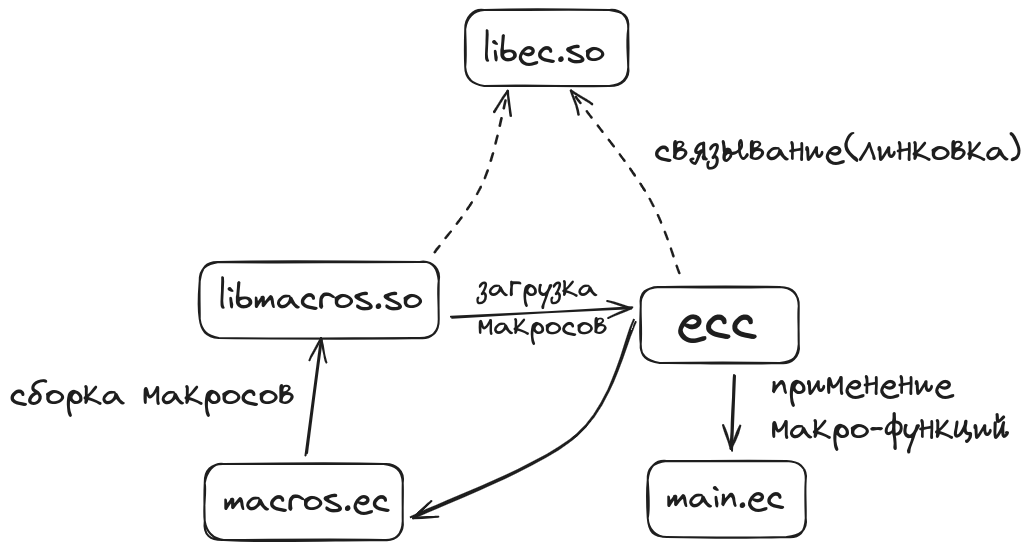
\includegraphics[width=\textwidth,height=\textheight,keepaspectratio]{macro-diag.png}
    \centering
    \caption{Процесс работы системы макро-функций}
    \label{pass:macros:diag}
\end{figure}
\FloatBarrier


% Термин символ в данном случае взят из терминологи линкера и означает упрощенно имя функции, переменной или в исходном коде языка(при условии, что компилятор не производит |name mangling|\cite{wiki:nm}).
% В случае языка Си, можно использовать это определение, т.к. он не производит изменения над именами функций(символами).
Термин символ в данном случае понимается как идентификатор, находящийся в таблице символов(аналогичной рассмотренной ранее[\ref{pass:parsing}]) линкера.
В случае языка Си это имя функции или переменной в исходном тексте программы, т.к. компилятор Си не производит изменение имен символов(\verb|name mangling|\cite{wiki-nm}).
В следующем листинге[\ref{pass:macros:macro-sym-diff}] имя символа - \verb|gen_dbg_fmt|, имя макро-функций, по которому она вызывается - \verb|DebugFormat|.

\begin{lstlisting}[language=c, caption={Заголовок функции gen\_dbg\_fmt}, label={pass:macros:macro-sym-diff}]
@derive_macro(DebugFormat)
ProcMacroError
gen_dbg_fmt(C_TranslationUnitData *data, C_Ast_Decl *decl, C_Ast_TranslationUnit **out_node);
\end{lstlisting}

Пример применения данной системы был рассмотрен выше[\ref{use-ex:code-gen}].


\subsection{Компиляция макросов}
\label{pass:macros:compile}
Рассмотрим процесс компиляции макросов подробнее.
Единица трансляции, в которой компилируются макросы отличается от обычной только тем, что в ней нет стадии применения макросов, 
что и понятно, ведь откуда их брать, если мы уже находимся в модуле, в котором все макро-функции должны быть. Все остальные стадии EC применяются.

Для этого этапа(прохода) в структуре \verb|TranslationUnitData| выделен блок[\ref{pass:macros:proc-macro-struct}].

\begin{lstlisting}[language=c, caption={Блок отвечающий за макро-функции}, label={pass:macros:proc-macro-struct}]
struct {
    hashmap_T(C_Symbol, EC_ProcMacroData) macros;
    void *lib; // handle from dlopen call

    void (*pm_init)();
    void (*pm_deinit)();
} proc_macro;
\end{lstlisting}

Данный блок содержит:
\begin{itemize}
    \item таблицу символов |macros|
    \item абстрактный указатель \verb|lib| на динамическую библиотеку, загружаемую в следующем параграфе[\ref{pass:macros:load}]
    \item указатели на динамически загружаемы функции инициализации и деинициализации динамически загружаемой библиотеки макросов
\end{itemize}


\begin{lstlisting}[language=c, caption={Структура содержащая информацию о символе макро-функции}, label={pass:macros:proc-macro-data-struct}]
enum_def(EC_ProcMacroKind,
    EC_PROC_MACRO_KIND_TRANSFORM,
    EC_PROC_MACRO_KIND_DERIVE,
    )

struct_def(EC_ProcMacroData, {
    EC_ProcMacroKind kind;
    str_t symbol_name;
    void *symbol;
})
\end{lstlisting}

Структура содержит информацию о:
\begin{itemize}
    \item типе символа \verb|kind|. На данный момент используется только тип \verb|DERIVE|
    \item имени символа \verb|symbol_name|
    \item указатель на машинный код символа в памяти \verb|symbol|
\end{itemize}
    
Привожу код функции отвечающей за компиляцию макросов:

\begin{lstlisting}[language=c, caption={Реализация функции компиляции макросов}, label={pass:macros:compile-impl}]
bool
ec_translation_unit_compile_macros(C_TranslationUnitData *self, C_BuildData *build_data) {
    if (self->string_arena.chunks == nullptr) {
        ASSERT_OK(arena_init(&self->string_arena, 4096, ctx_global_alloc));
    }

    C_TranslationUnitData macro_tr_unit;
    c_translation_unit_init(&macro_tr_unit, build_data->macro_path);
    ASSERT(c_translation_unit_lex(&macro_tr_unit));
    ASSERT(ec_translation_unit_parse(&macro_tr_unit));
    ASSERT(ec_translation_unit_collect_proc_macro_names(&macro_tr_unit, 
        arena_allocator(&self->string_arena), &self->proc_macro.macros));

    WITH_FILE(build_data->macro_tmp_c_path, "w", file, {
        OutputFileStream ofs;
        ASSERT_OK(file_sw(file, &ofs));
        auto sw = output_file_stream_stream_writer(&ofs);
        ec_translation_unit_ast_compile_c(&macro_tr_unit, &sw);
    })
    auto string_alloc = arena_allocator(&self->string_arena);
    String s;
    ASSERT_OK(string_new_cap_in(128, &string_alloc, &s));
    sprint_fmt(&s, S("%s %s -fPIC -shared -Wall -o %s -std=c2x -g -Wall -I. -I./lib -L./build -lec\0"), 
        build_data->cc_path, build_data->macro_tmp_c_path, build_data->macro_lib_path);
    s.byte_len -= 1;
    str_t build_cmd = string_to_str(&s);

    if (system((char *)build_cmd.ptr) != 0) { return false; }
    
    c_translation_unit_deinit(&macro_tr_unit);

    return true;
}
\end{lstlisting}

Как можно видеть сначала файл с макросами, полученный из \verb|build_data|, сначала преобразуется к AST, 
функциями \verb|c_translation_unit_lex| и \verb|ec_translation_unit_parse|, 
рассмотренных ранее в соответствующих главах лексического[\ref{pass:lexing}] и грамматического разбора[\ref{pass:parsing}].

К полученному AST далее применяется проход \verb|ec_translation_unit_collect_proc_macro_names|, 
который строит таблицу(заполняет) таблицу символов макро-функций[\ref{pass:macros:proc-macro-struct}], 
собирая имена макро-функций и имена символов, реализующие их.
Делает она это путем интерпретации директив(на данный момент только \verb|@derive_macro|).

После формирования таблицы символов для макро-функций, выполняется трансляция AST к коду языка Си функцией \verb|ec_translation_unit_ast_compile_c|, 
разобранной ранее[\ref{pass:compile-c}]. Полученный код языка Си записывается в выходной промежуточный файл средствами типа \verb|OutputFileStream|.

Наконец промежуточный файл с кодом макро-функций на языке Си компилируется в динамическую библиотеку с помощью компилятора, 
предоставленного системой(в данном прототипе используется \verb|gcc|).
При этом происходит связывание(линковка) данной библиотеки макро-функций с библиотекой \verb|ec.so|.

Если на каком-то этапе выполнения некоторая подфункция вернет ошибку, то вся функция возвращается с ошибкой, возвращая |false|.

\subsection{Динамическая загрузка макросов}
\label{pass:macros:load}

После получения динамической библиотеки макро-функций(назовем \verb|libmacros.so|) выполняется динамическая загрузка библиотеки в виртуальную память процесса компилятора \verb|ecc|.
Далее привожу код[\ref{pass:macros:load-impl}] функции \verb|ec_translation_unit_load_macro_symbols|, выполняющей данную операцию. 

\begin{lstlisting}[language=c, caption={Реализация функции загрузки макросов}, label={pass:macros:load-impl}]
bool
ec_translation_unit_load_macro_symbols(C_TranslationUnitData *self, str_t libmacros_path) {
    ASSERT(self->proc_macro.macros != nullptr);

    auto string_alloc = arena_allocator(&self->string_arena);
    str_t lib_path;
    ASSERT_OK(str_null_terminate_in(libmacros_path, &string_alloc, &lib_path));

    void *lib = dlopen((char *)lib_path.ptr, RTLD_NOW);
    if (!lib) {
        fprintf(stderr, "dlopen failed: %s\n", dlerror());
        return false;
    }
    self->proc_macro.lib = lib;
    
    void *pm_init = dlsym(lib, "proc_macro_init");
    void *pm_deinit = dlsym(lib, "proc_macro_deinit");
    if (pm_init == nullptr) {
        fprintf(stderr, "dlsym for proc_macro_init failed: %s\n", dlerror());
        return false;
    }
    if (pm_deinit == nullptr) {
        fprintf(stderr, "dlsym for proc_macro_deinit failed: %s\n", dlerror());
        return false;
    }
    self->proc_macro.pm_init = pm_init;
    self->proc_macro.pm_deinit = pm_deinit;

    bool was_err = false;
    for_in_range(i, 0, hashmap_len(self->proc_macro.macros)) {
        auto val = slice_get_T(EC_ProcMacroData, &self->proc_macro.macros->values, i);
        // symbol_name is assumed to be null-terminated
        void *macro = dlsym(lib, (char *)val->symbol_name.ptr);
        if (macro == nullptr) {
            fprintf(stderr, "dlsym for %s failed: %s\n", (char *)val->symbol_name.ptr, dlerror());
            was_err = true;
        }
        val->symbol = macro;
    }
    if (was_err) {
        return false;
    }

    return true;
}
\end{lstlisting}

В настоящем прототипе загрузка выполняется средствами \verb|glibc| \verb|dlopen| и \verb|dlsym|.

Сначала символы динамической библиотеки подгружаются в память текущего процесса вызовом \verb|dlopen|(строка 9, \ref{pass:macros:load-impl}).
Далее разрешаются указатели на них вызовами \verb|dlsym|.

Подразумевается, что в библиотеке \verb|libmacros.so| присутствуют символы инициализации \verb|proc_macro_init| и деинициализации \verb|proc_macro_deinit| библиотеки макросов, 
на данный момент они определены в заголовочном файле \verb|proc_macro.h|(тот, что был в примере макро-функции вывода[\ref{use-ex:macro-file}]).
Их символы подгружаются в отведенный блок[\ref{pass:macros:proc-macro-struct}] структуры \verb|TranslationUnitData|.

Далее для каждой позиции в таблице символов макро-функций, полученной ранее на этапе компиляции макросов[\ref{pass:macros:compile}], 
разрешается указатель на соответствующий данному макросу символ.

Если какой-то символ не может быть разрешен, то функция данная функция[\ref{pass:macros:load-impl}] выдает ошибку.

\subsection{Применение макросов}
\label{pass:macros:apply}

Теперь, когда у нас есть таблица макро-функций с загруженными символами, мы можем применить макро-функции в коду основного модуля(единицы трансляции),
это делается после получения AST из кода основного модуля с помощью интерпретации директив.

Привожу код[\ref{pass:macros:apply-impl}] функции интерпретирующей директивы применения макро-функций(на данном этапе выполнена только директива \verb|@derive|):
\begin{lstlisting}[language=c, caption={Реализация функции применения макросов}, label={pass:macros:apply-impl}]
bool
ec_translation_unit_apply_proc_macros(C_TranslationUnitData *self) {
    ASSERT(self->proc_macro.macros);

    auto tr_unit = (EC_Ast_TranslationUnit *)self->tr_unit;
    if (darr_len(tr_unit->items) == 0) {
        return true;
    }
    auto ast_alloc = arena_allocator(&self->ast_arena);
    darr_t processed = nullptr;
    ASSERT_OK(darr_new_cap_in_T(EC_Ast_TrUnitItem *, darr_len(tr_unit->items), &ast_alloc, &processed));

    self->proc_macro.pm_init();

    for_in_range(i, 0, darr_len(tr_unit->items)) {
        auto item = *darr_get_T(EC_Ast_TrUnitItem *, tr_unit->items, i);
        if (item->kind == C_AST_NODE_KIND_DECL) {
            ASSERT_OK(darr_push(&processed, &item));
            continue;
        }
        ASSERT(item->kind == C_AST_NODE_KIND_AT_DIRECTIVE);

        auto name = item->at_directive.name->name;
        if (str_eq(name, S("derive"))) {
            if (i == darr_len(tr_unit->items)-1) {
                eprint_fmt(S("stray @derive macro invocation\n"));
                return false;
            }
            if (item->at_directive.args == nullptr || darr_len(item->at_directive.args) < 1) {
                eprint_fmt(S("@derive expects at least one argument\n"));
                return false;
            }

            auto next = *darr_get_T(EC_Ast_TrUnitItem *, tr_unit->items, i+1);
            if (next->kind != C_AST_NODE_KIND_DECL) {
                eprint_fmt(S("@derive expects declaration\n"));
                return false;
            }
            ASSERT_OK(darr_push(&processed, &next));
            for_in_range(j, 0, darr_len(item->at_directive.args)) {
                auto arg = *darr_get_T(C_Ast_Node *, item->at_directive.args, j);
                if (arg->kind != C_AST_NODE_KIND_IDENT) {
                    eprint_fmt(S("@derive expects arguments of type C_Ast_Ident\n"));
                    return false;
                }
                
                auto data = hashmap_get_T(EC_ProcMacroData, self->proc_macro.macros, &arg->ident.name);
                if (data == nullptr) {
                    eprint_fmt(S("there is no such macro %s\n"), arg->ident.name);
                    return false;
                }
                DeriveMacroFn *macro = (DeriveMacroFn *)data->symbol;
                C_Ast_TranslationUnit *res = nullptr;
                if (IS_ERR(macro(self, (C_Ast_Decl *)next, &res))) {
                    eprint_fmt(S("%s macro failed\n"), arg->ident.name);
                    return false;
                }
                ASSERT_OK(darr_append_slice(&processed, darr_slice_full(res->decls)));
            }
            i += 1;
        } else {
            ASSERT_OK(darr_push(&processed, &item));
            continue;
        }
    }

    self->proc_macro.pm_deinit();
    tr_unit->items = processed;
    return true;
}
\end{lstlisting}

При применении макро-функций первым делом надо инициализировать библиотеку макросов, делается это вызовом символа \verb|proc_macro_init|, который подгружен в указатель \verb|pm_init|.

После обработки новый список определений будет содержаться в динамическом массиве \verb|processed|.

Далее последовательно итерируем по списку корневых определений, определения без примененных к ним директив просто записываем в выходной массив.
При нахождении директивы интерпретируем ее следующим образом:
\begin{enumerate}
    \item проверяем существования определения, к которому должна быть применена директива
    \item проверяем, что в макро-функцию подавался хотя бы один аргумент
    \item проверяем, чтобы синтаксический тип аргументов, подаваемых в функцию, был \verb|C_Ast_Ident|
    \item загружаем соответствующий данному имени макроса символ из таблицы макросов \verb|proc_macro.macros| структуры \verb|TranslationUnitData|
    \item применяем полученный символ к последующему определению, получаем результат в виде типа \verb|C_Ast_TranslationUnit|
    \item добавляем определения из полученной AST единицы трансляции в выходной массив определений \verb|processed|
\end{enumerate}


По окончанию работы с библиотекой деинициализируем ее вызовом функции по указателю \verb|pm_deinit|.

Таким образом были рассмотрены все подсистемы, входящие в состав системы макро-функций.